\documentclass{article}
\usepackage[top=1in, bottom=1in, left=1in, right=1in]{geometry}
\usepackage{amsmath}
\usepackage{booktabs}
\usepackage{graphicx}
\usepackage{caption}
\usepackage{wrapfig}

\graphicspath{ {../media/} }

\begin{document}
\section*{RESULTS}

\begin{wrapfigure}{L}{3in}
\begin{tabular}{| c c c c |}
	\toprule
	Mixtures      	     &  A    & B    &  C \\
	\midrule
	Ethanol (ml)  	 	 &  2    & 2    &  3 \\
	Water   (ml)  	 	 & 10    & 8.3  &  7 \\
	Concentration (mols) & 12 ml & 10.3 & 10 \\
   	Index         		 & N/A   & N/A  & N/A \\
	\bottomrule
\end{tabular}
\end{wrapfigure}
The table to the left lists the mixtures of ethanol used to test for a change in index of refraction (*This initial data is poorly measured and more data is being taken*). The plot below shows the different indices of refraction corresponding to mixture A being injected over the interval $[45.0, 55.0]$. Similarly mixture B was injected over the interval $[60.0, 75.0]$, and mixture C over $[85.0, 95.0]$. The dip in mode position is not expected over the first two intervals as we expect the mode to shift horizontally if the index of refraction in the chamber becomes larger than the original. However, the water used had been sitting in a syringe for a few days and may have actually increased in index of refraction, meaning that the index of the water in the chamber before injecting the first mixture may have been higher than the first two mixtures.
\begin{wrapfigure}{R}{4in}
	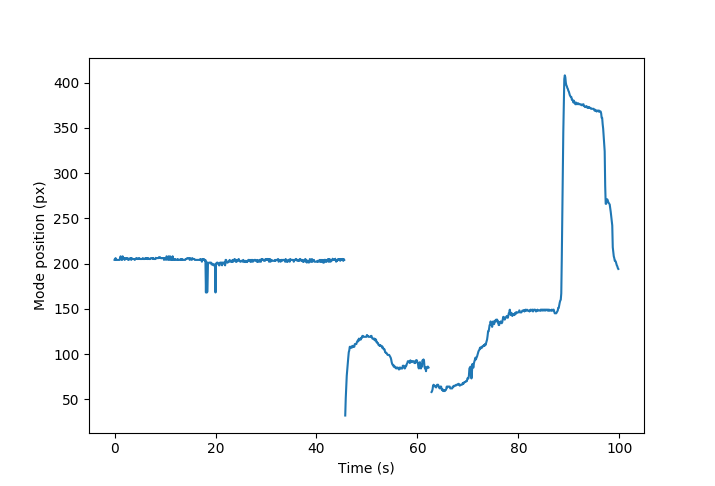
\includegraphics[width=4in]{mode_position_3-21-2019.png}
\end{wrapfigure}

From this data we can infer a change in index of refraction of the medium once the index values of each mixture is known. Although we do not know the index of refraction we do know that the biosensor is highly sensitive as the index of ethanol is about $1.36$ and water is $1.33$ so our device is registering a change in index of at least $10^{-3}$.


\end{document}
